
%----------------------------------------------------------------------------------------------------------
\clearpage
\section{Fragmentation function and \xe}

Variable \xe{} is defined as
\begin{equation}
\xe{} = - { \vec{p}_{\rm Ta}\cdot \vec{p}_{\rm Tt}   \over \ptt{}^{2}} =-{\pta{} \over \ptt{}} \cos\Delta\phi 
\simeq \frac{\za\ptq{a}}{\zt\ptq{t}} \big|_{\dphi\rightarrow\pi}
\simeq \frac{\za}{\zt} \big|_{\dphi\rightarrow\pi\wedge\kt{}\rightarrow 0}
\simeq \za \big|_{\dphi\rightarrow\pi\wedge\kt{}\rightarrow 0\wedge\zt\rightarrow 1}
\label{eq:xE} 
\end{equation} 
For back-to-back pairs ($\dphi\rightarrow\pi$) \xe\ is equal to the ratio $\za\ptq{a}/\zt\ptq{t}$. For small values of \kt{} when $\ptq{a}\simeq\ptq{t}$, \xe\ variable reflects the ratio \za/\zt.  Since 1970s It has been believed that the \xe{} distribution associated to the high-\pt{} charged particle or \piz\ reflects directly the fragmentation function \cite{CCOR_xe}. Why this was generally adopted  is evident from 
the last term of \eq{eq:xE}. If f \zt\ is sufficiently close to unity then $\xe\simeq\za$ and thus the \xe{} distribution has the same shape as the fragmentation function. There are good reasons for these assumption known as a "trigger bias" \cite{Jacob:1978mj} 
and the "Bjorken Parent-Child Relationship"  (PCR) \cite{Bjorken:1973kd}. More details follows in section \ref{sec:parent-child}.

The simulation is done in following steps:
\begin{enumerate}
\item Generate the di-jet four-momenta $(\ptq, 0,\ptq{})$, $(\ptq, 0,-\ptq{})$ in c.m. system by sampling from a flat distribution ((E,$p_{||}, \vpt{})$ notation). 
\item Generate random net-pair momentum \pn{} according 2D Gaussian of the variance $\sigma_{\pn}=\sqrt{2\rms{\kt{}}}$.
\item Apply a Lorentz boost to the back-to-back parton pair according formula given below.
\item Generate random \zt{} according Leading Particle (LP) fragmentation function according \eq{eq:LPFF}
\item Generate random \za{} according KKP fragmentation function according \eq{eq:FF}
\item Generate random \jt{} component and add it to calculated particle \pt{t,a} = $z_{t,a}\ptq{t,a}+\jt{}\cdot\vec{e}_{\perp}$
\end{enumerate}

Toy simulations (see \ref{sec:intro} and \fig{fig:gamma}) clearly demonstrates the connection between fragmentation function and the \xe\ distribution when the trigger  particle is identical to trigger jet (\zt=1.0 as it is in the case of the direct-$\gamma$ and \kt{}=0 \gevc) . When the away side jet is emitted at the angle different from $\pi$ then the \xe\ distribution becomes steeper. 
\begin{figure}[htbp]
   \centering
   %\resizebox{0.49\columnwidth}{!}{\includegraphics[viewport=54 56 456 821,clip=]{}} 
   \subfigure[]{ \label{fig:gamma}   \resizebox{0.48\columnwidth}{!}{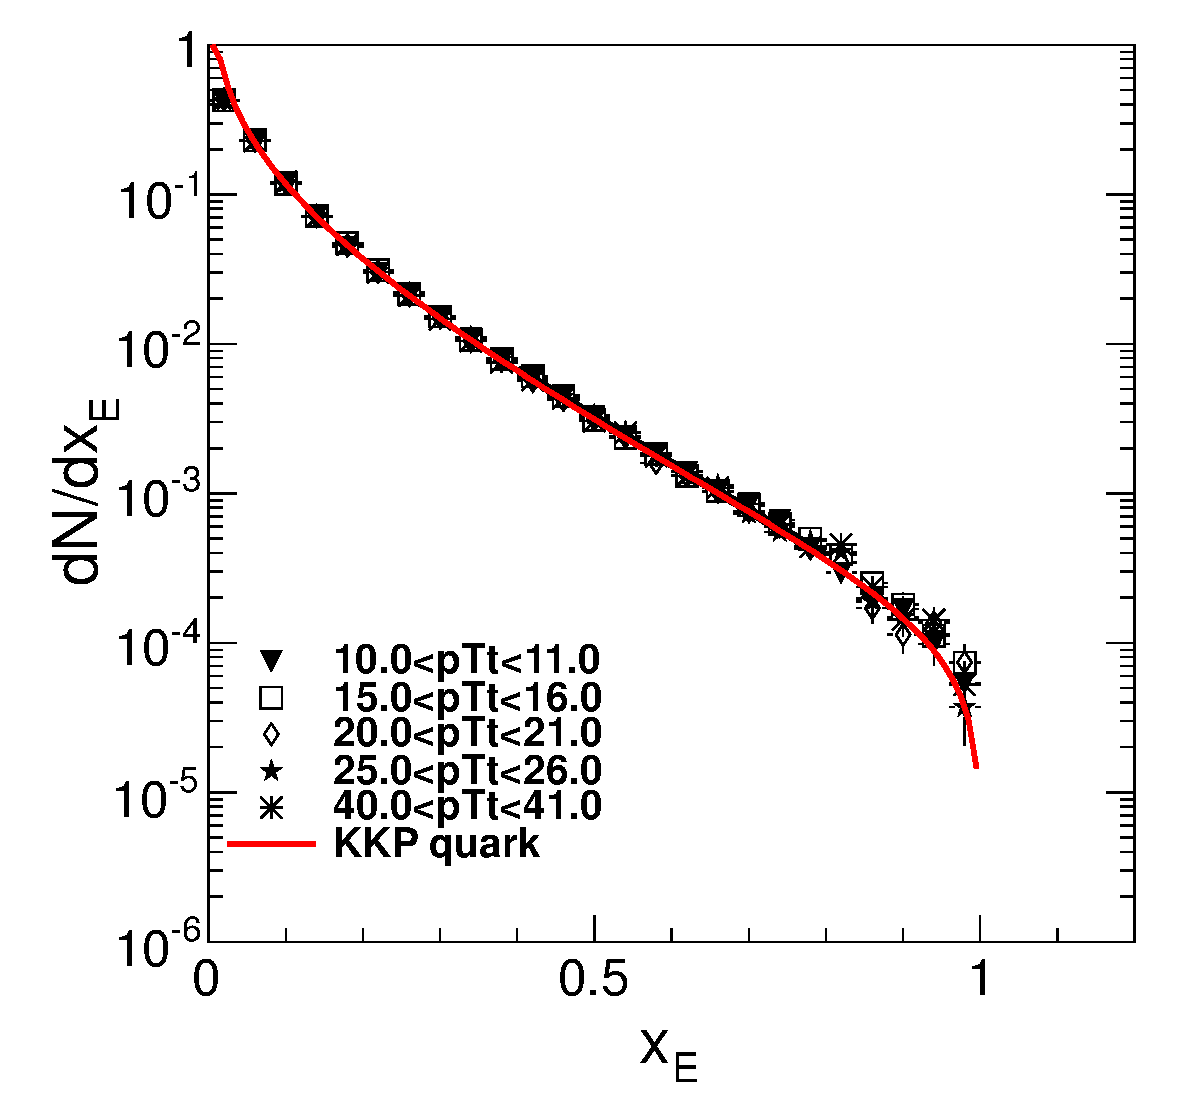
\includegraphics{xe_gamma_q}} }
   \subfigure[]{ \label{fig:gamma3pi4} \resizebox{0.48\columnwidth}{!}{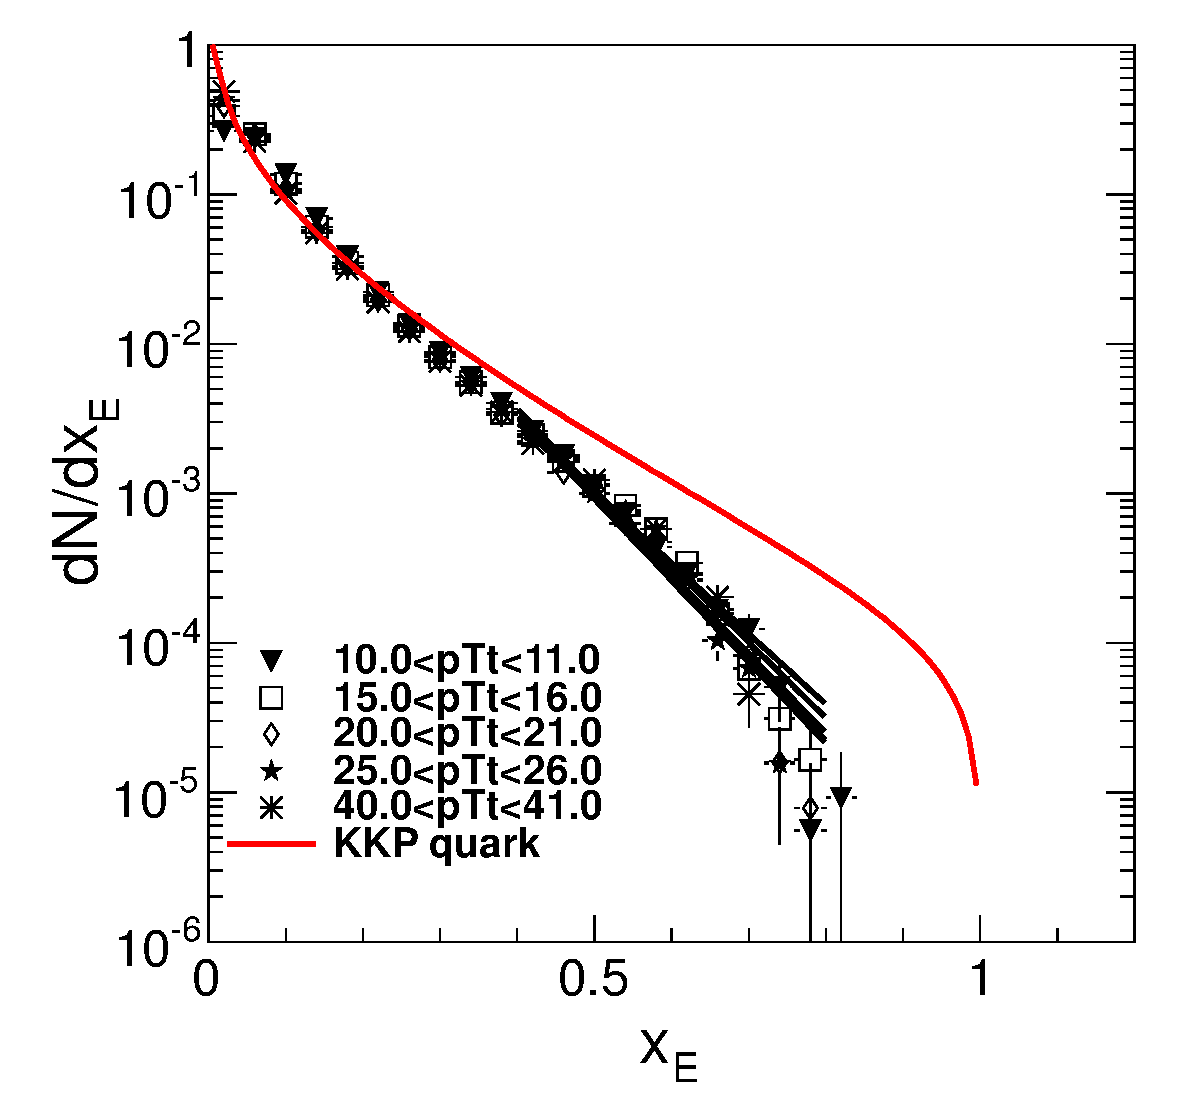
\includegraphics{xe_gamma_3pi4}} }
   \caption{Left: \xe{} distributions from the toy simulations with KKP parameterization \eq{eq:FF} of the quark  fragmentation function and 
   \zt=1.0 as it is e.g. in the case of $\gamma$-hadron correlations. An effect of \kt{} smearing is mimicked by away-side emission 
    at an angle $\dphi = 3\pi/4$ w.r.t. trigger jet shown on the right panel.}  
\end{figure}
\begin{figure}[htbp]
   \centering
   %\resizebox{0.49\columnwidth}{!}{\includegraphics[viewport=54 56 456 821,clip=]{}} 
   \subfigure[]{ \label{fig:gamma_qg}   \resizebox{0.48\columnwidth}{!}{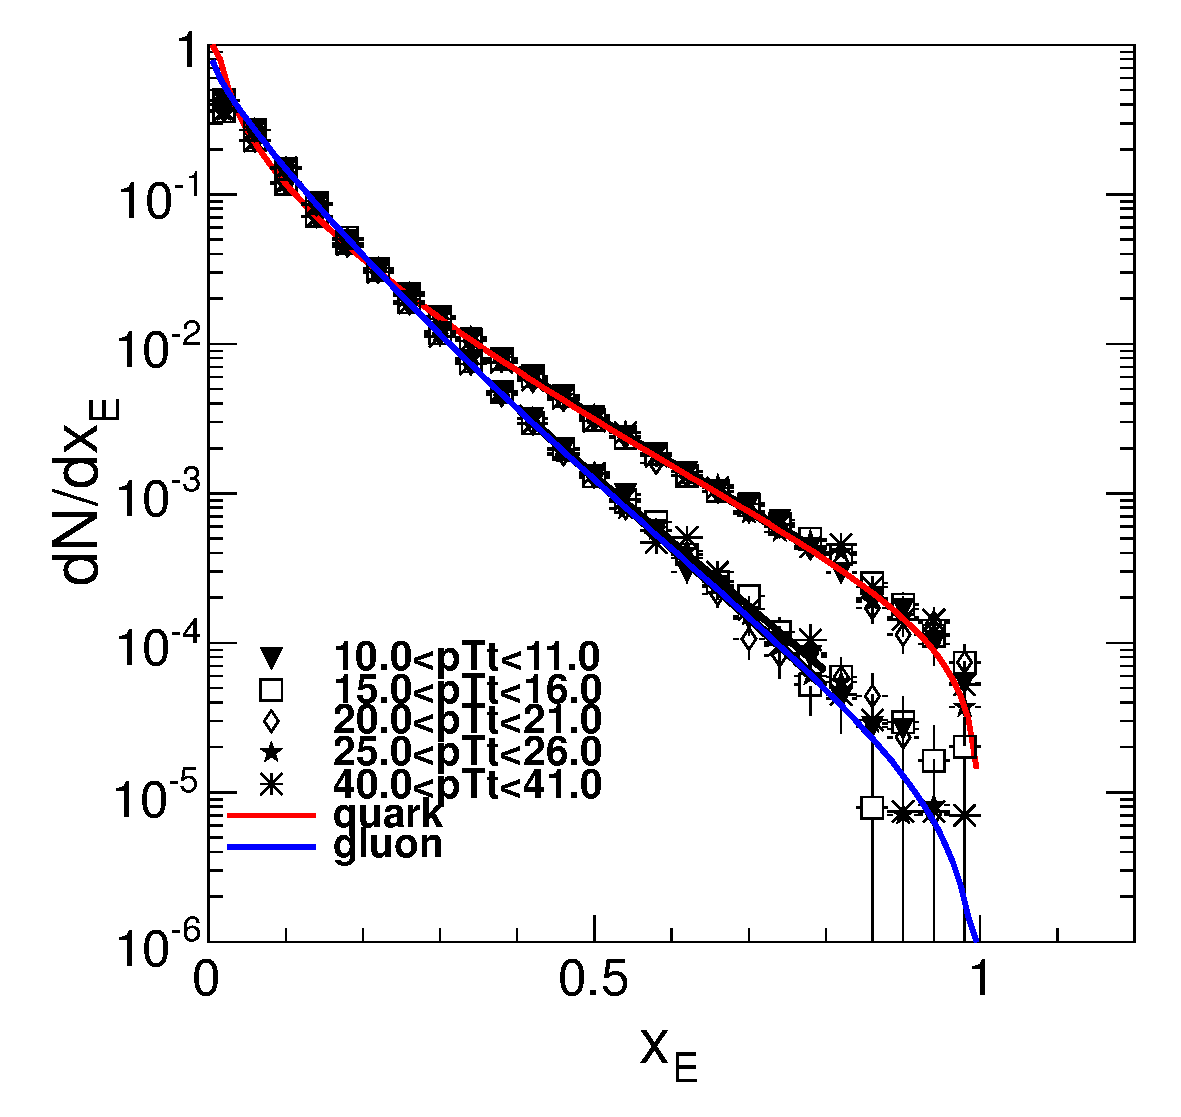
\includegraphics{xe_gamma_qg}} }
   \subfigure[]{ \label{fig:gamma_hh}   \resizebox{0.48\columnwidth}{!}{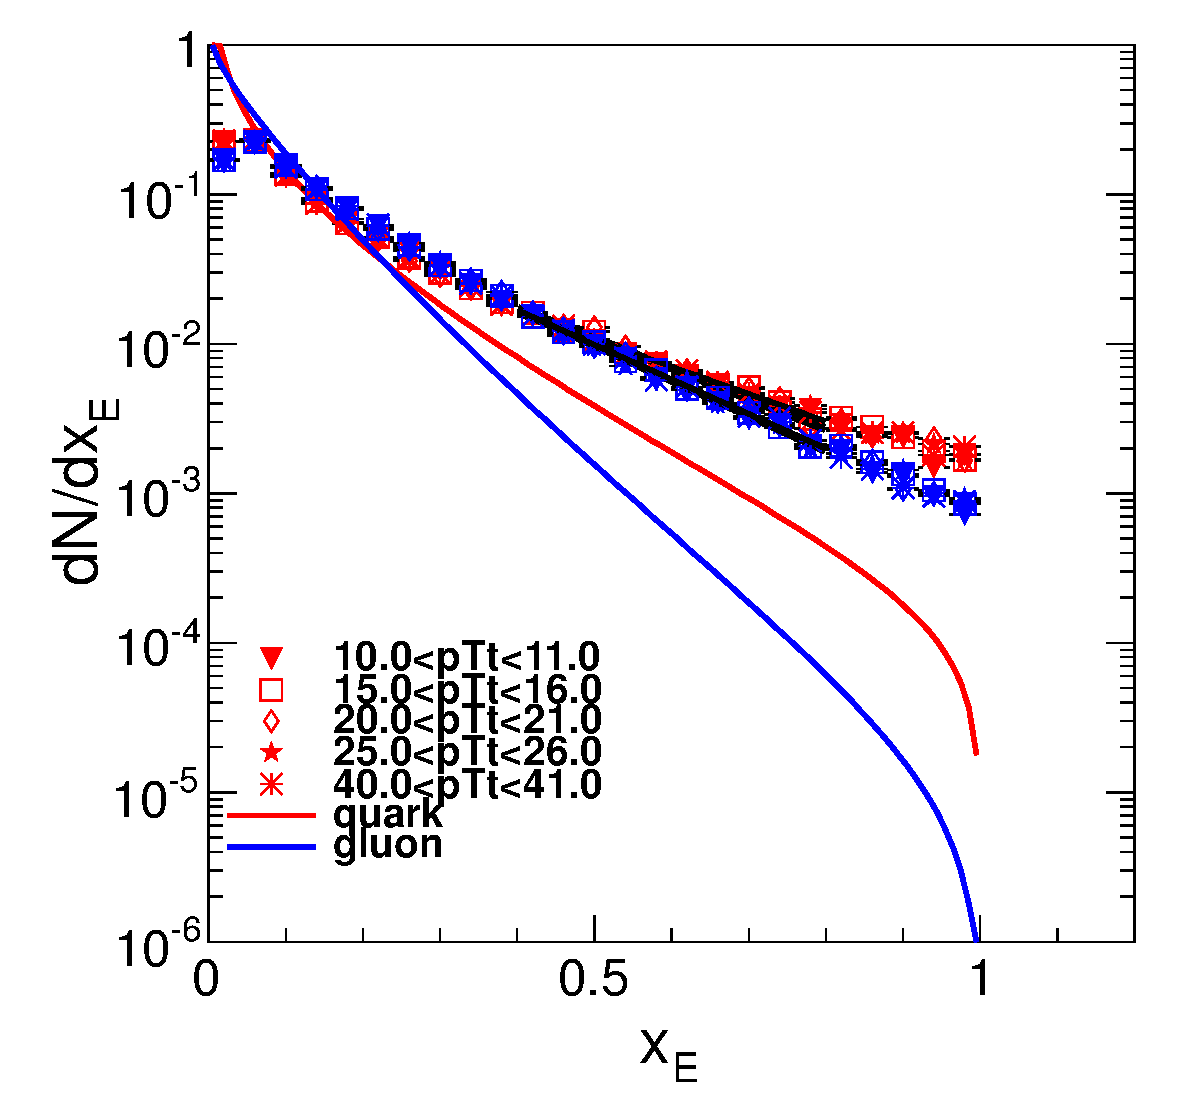
\includegraphics{xe_dihad_qg}} }
   \caption{Left: \xe{} distributions from the toy simulations with KKP parameterization \eq{eq:FF} of the quark and gluon fragmentation 
   function, \zt=1.0 and \kt{}=0 \gevc. Righ: the same \xe-distributions as on the left panel but the trigger is a fragment carrying $\zt<1$ 
   (leading particle fragmentation according \eq{eq:LPFF}).}  
\end{figure}
This demonstrated at 
\fig{fig:gamma3pi4} where an effect of \kt{} smearing is mimicked by away-side particle emission at angle $\dphi = 3\pi/4$ w.r.t. trigger jet.
One can observe an enhancement the low-\xe{} part and increases the high-\xe{} slope.
Figure \ref{fig:gamma_qg} shows the simulated \xe-distributions with KKP parameterization \eq{eq:FF} of the quark and gluon 
fragmentation  function and \zt=1.0. Obviously in the case of no \kt-smearing the \xe-distribution follow exactly the fragmentation function.
However, when the trigger particle is a fragmented hadron carrying $\zt<1$ (\fig{fig:gamma_hh}) then the \xe{} distributions becomes flatter and the sensitivity to the actual shape of the fragmentation function is, to the large extend, suppressed.


\begin{figure}[htbp]
   \centering
   %\resizebox{0.49\columnwidth}{!}{\includegraphics[viewport=54 56 456 821,clip=]{}} 
   \subfigure[]{ \label{fig:gamma34} \resizebox{0.48\columnwidth}{!}{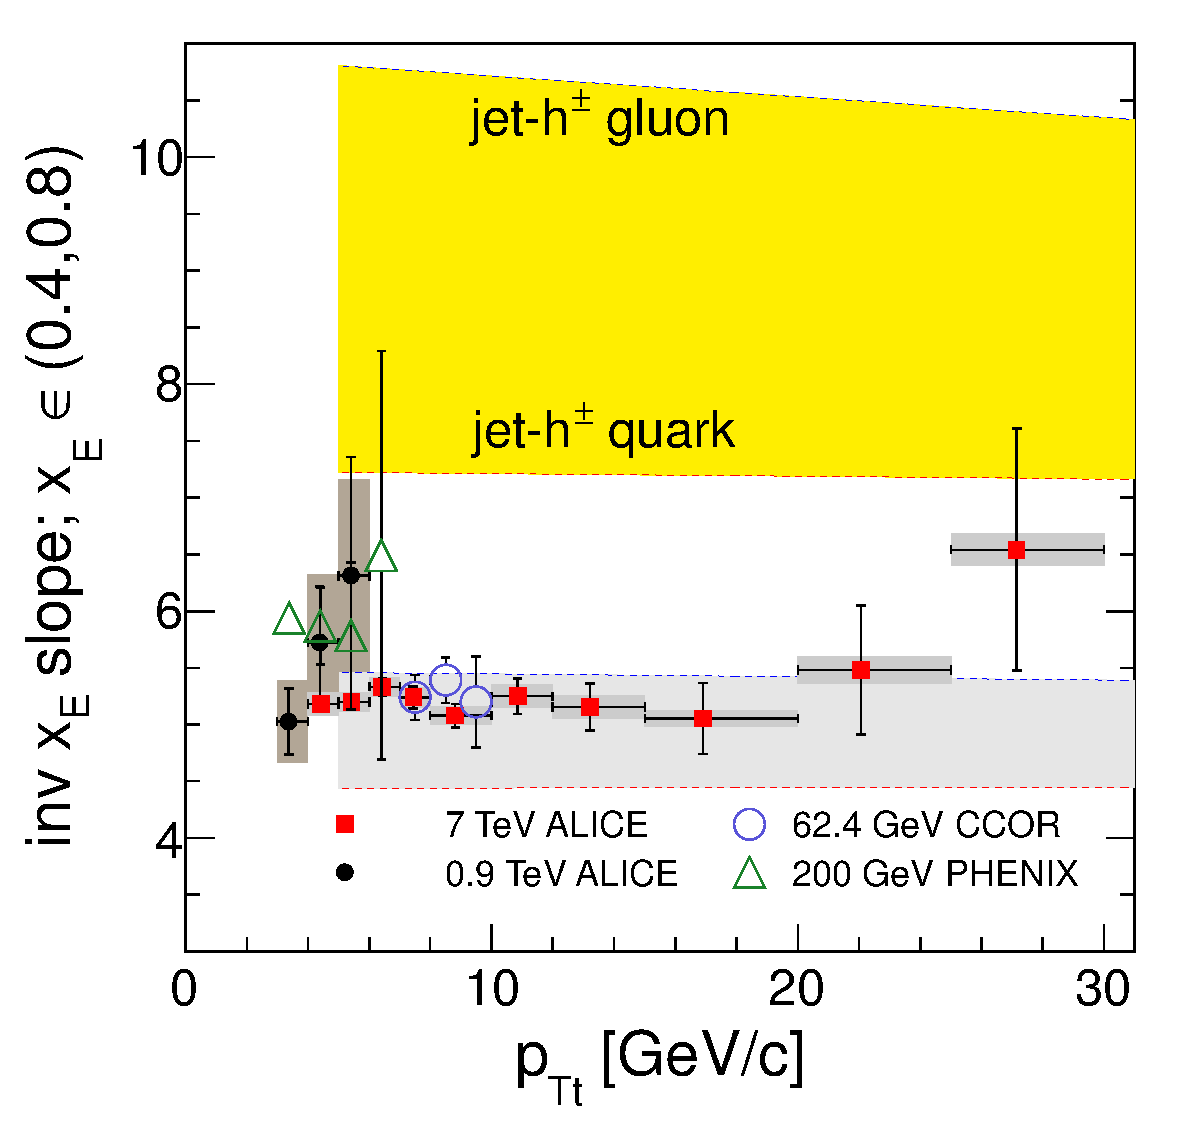
\includegraphics{pap_invXeSlope}} }
   \caption{\xe{} distributions in the case the away-side jets is emitted at an angle $\dphi = 3\pi/4$ w.r.t. trigger jet and fixed \zt=1.0}  
\end{figure}


\clearpage
\section{Various}

Generally, a conditional probability of parton \ptq{} fragmenting into a particle \pt{} can be written
\begin{equation}\label{eq:child}
\frac{dP}{d\pt{}}\Biggl\vert_{\ptq{}} = D\left(\frac{\pt{}}{\ptq{}}\right)\frac{dz}{\pt{}} = D\left(\frac{\pt{}}{\ptq{}}\right)\frac{1}{\ptq{}}
\end{equation}
and thus \pt{} distribution has the same shape as the fragmentation function. 
Conditional probability of particle \pt{} being a fragment of parton \ptq{} can be written
\begin{equation}\label{eq:parent}
\frac{dP}{d\ptq{}}\Biggl\vert_{\pt{}} = 
       \frac{dP}{d\ptq{}} \frac{dP}{d\pt{}}\Biggl\vert_{\ptq{}} \frac{d\ptq{}}{d\pt{}}= 
       \ptq{}^{-n} D\left(\frac{\pt{}}{\ptq{}}\right)\frac{1}{\pt{}}\ .
\end{equation}
Two examples of the parton distributions fragmenting into a \pt{}=10 \gevc\ particle are shown on \fig{fig:paret-child}. Final state parton spectrum is simulated according the $\ptq{}^{-6}$ and the fragmentation function is a simple exponential function $D(z)=\exp(-6z)$ (left panel) or parameterization \eq{eq:LPFF} (right panel). Lines represent \eq{eq:parent}.
\begin{figure}[htbp]
   \centering
   %\resizebox{0.49\columnwidth}{!}{\includegraphics[viewport=54 56 456 821,clip=]{}} 
   \resizebox{0.49\columnwidth}{!}{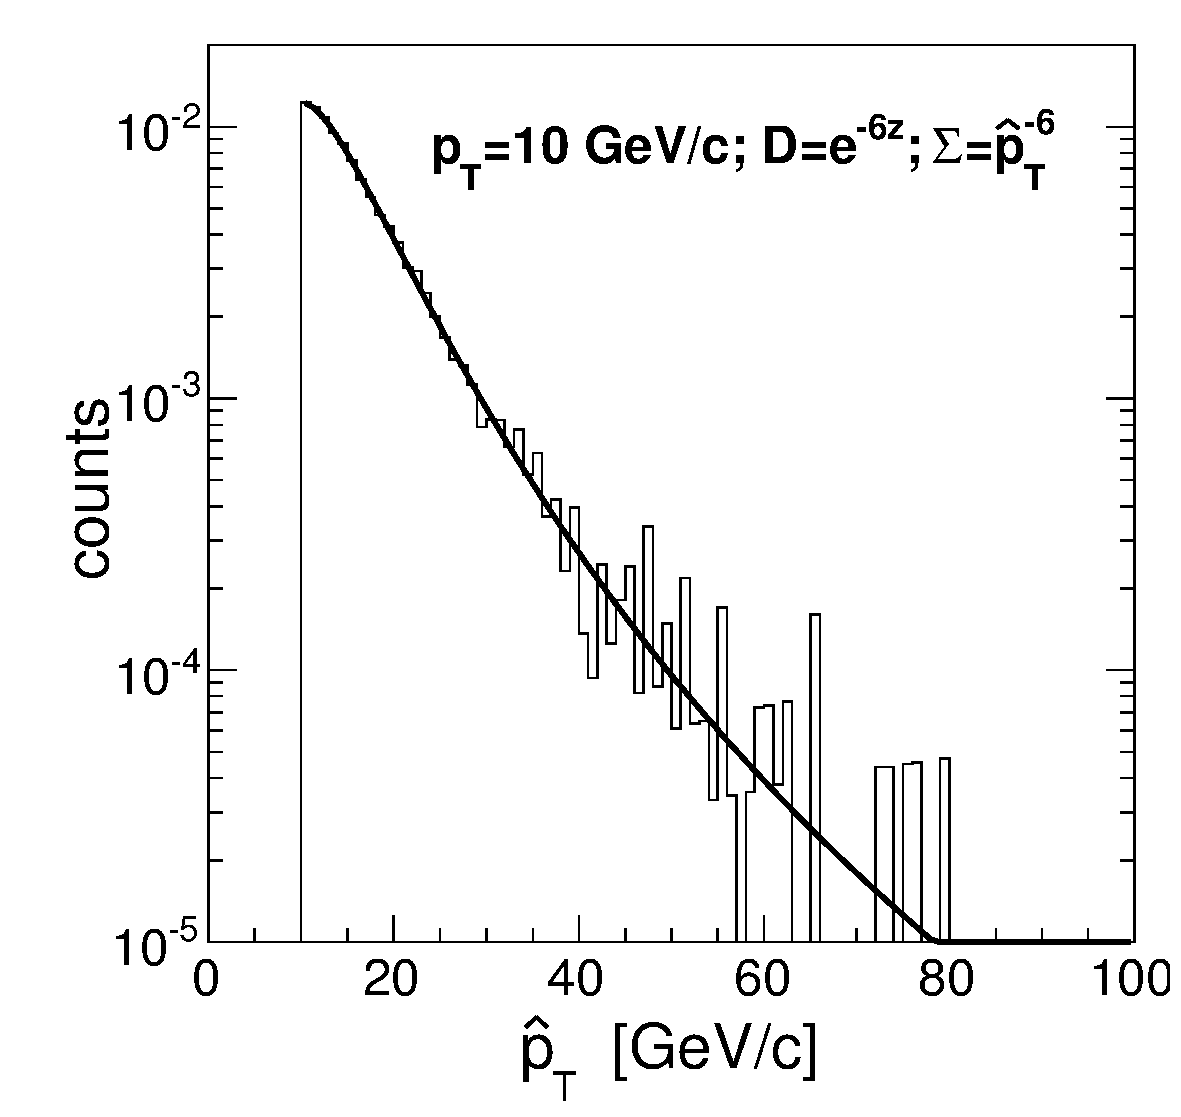
\includegraphics{fig-p-c}} 
   \resizebox{0.49\columnwidth}{!}{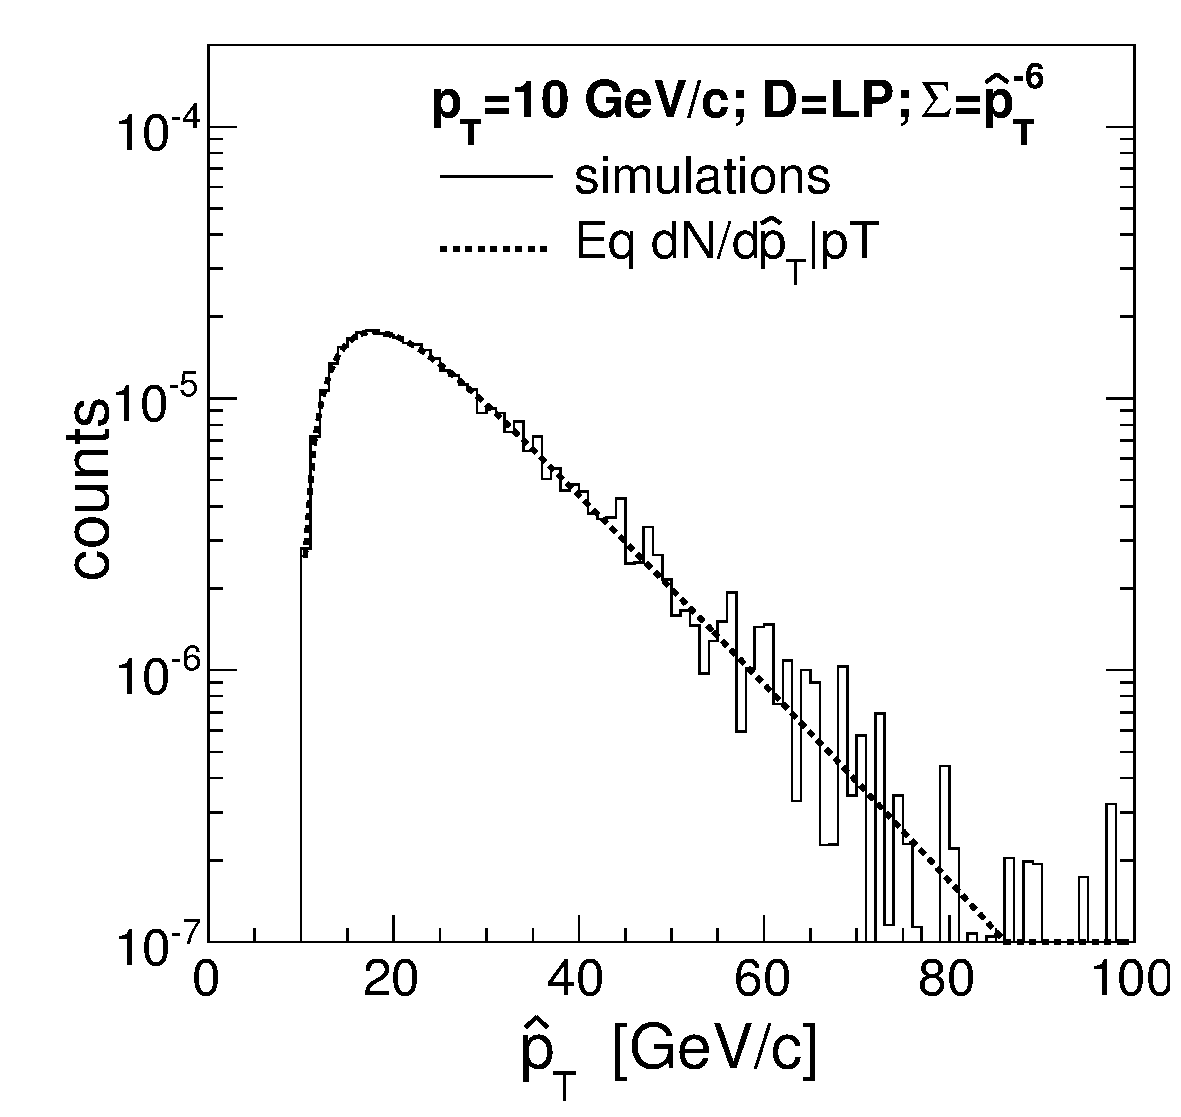
\includegraphics{fig-p-c-LP}} 
   \caption{Distribution of parent partons fragmenting into a 10 \gevc\ hadron from the toy simulation and \eq{eq:parent} (dashed line).
   Distribution of inclusive partons according power law $dN/d\ptq{}\propto\ptq{}^{-6}$ and the fragmentation function $D(z)\approx\exp(-6z)$ 
   (left panel) or leading particle fragmentation function according \eq{eq:LPFF} (right panel).
   }  
   \label{fig:paret-child}
\end{figure}

\section{Fragmentation function and \kt{}}

